\documentclass{article}
\usepackage[T1]{fontenc}
\usepackage[polish]{babel}
\usepackage[utf8]{inputenc}
\usepackage{graphicx} % Required for inserting images
\usepackage{amsmath}
\usepackage{float}
\DeclareMathOperator{\cond}{cond}
\DeclareMathOperator{\ctg}{ctg}

\title{MOwNiT - Laboratorium 1: \\
Arytmetyka komputerowa}
\author{Wojciech Dąbek}
\date{5 marca 2024}

\begin{document}

\maketitle

\section{Treści zadań}

\begin{enumerate}
    \item Znaleźć \textit{"maszynowe epsilon"}, czyli najmniejszą liczbę \textit{a}, taką że \(a+1>1\).
    \item Rozważamy problem ewaluacji funkcji \(sin(x)\), m.in. propagację błędu danych wejściowych, tj. błąd wartości funkcji ze względu na zakłócenie \textit{h} w argumencie \textit{x}:
    \begin{itemize}
        \item Ocenić błąd bezwzględny przy ewaluacji \(sin(x)\).
        \item Ocenić błąd względny przy ewaluacji \(sin(x)\)
        \item Ocenić uwarunkowanie dla tego problemu
        \item Dla jakich wartości argumentu \textit{x} problem jest bardzo czuły?
    \end{itemize}
    \item Funkcja sinus zadana jest nieskończonym ciągiem:
    \[sin(x) = x - \frac{x^3}{3!} + \frac{x^5}{5!} - \frac{x^7}{7!} + \ldots\]
    \begin{itemize}
        \item Jakie są błędy progresywny i wsteczny jeśli przybliżamy funkcję sinus biorąc tylko pierwszy człon rozwinięcia,\\
        tj. \(sin(x) \approx x\), dla \(x = 0.1, 0.5\) i \(1.0\)?
        \item Jakie są błędy progresywny i wsteczny jeśli przybliżamy funkcję sinus biorąc pierwsze dwa człony rozwinięcia,\\
        tj. \(sin(x) \approx x - \frac{x^3}{6}\), dla \(x = 0.1, 0.5\) i \(1.0\)?
    \end{itemize}
    \item Zakładamy że mamy znormalizowany system zmiennoprzecinkowy\\
    z \(\beta = 10, p = 3, L = -98\).
    \begin{itemize}
        \item Jaka jest wartość poziomu UFL (underflow) dla takiego systemu?
        \item Jeśli \(x = 6.87 \cdot 10^{-97}\) i \(y = 6.81 \cdot 10^{-97}\), jaki jest wynik operacji \(x - y\)?
    \end{itemize}
\end{enumerate}

\section{Rozwiązania}

\subsection{}
Przyjmując definicję \textit{maszynowego epsilonu} z polecenia będzie on równy wartości "jednostki ostatniego miejsca"\ względem 1, czyli wartości przyjmowanej, gdy mantysa jest równa 1 (najmniejsza), a wykładnik taki jak dla 1.\\
Zatem:
\[\varepsilon = b^{1 - p}\]
gdzie \textit{b} jest podstawą systemu liczbowego, a \textit{p} precyzją.

\vspace{3mm}
\noindent
Przykładowo dla wartości typu \textit{double} w języku C++ stosowana jest\\
podstawa 2 i precyzja 53, więc \(\varepsilon = 2^{-52} \approx 2,22 \cdot 10^{-16}\).

\subsection{}
\begin{itemize}
    \item Błąd bezwzględny:
    \[\Delta \sin x = |\sin x - \sin(x(1 + \varepsilon))|\]
    \item Błąd względny:
    \[\frac{\Delta \sin x}{\sin x} = \frac{|\sin x - \sin(x(1 + \varepsilon))|}{\sin x}\]
    \item Uwarunkowanie:
    \[\cond (\sin x) = \left|\frac{x \sin'x}{\sin x}\right| = \left|\frac{x \cos x}{\sin x}\right| = |x \ctg x|\]
    \begin{figure}[H]
        \centering
        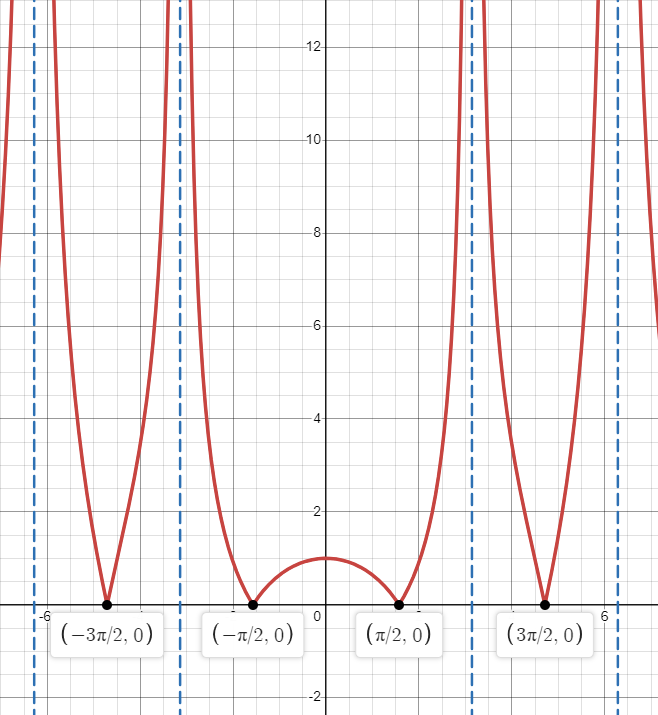
\includegraphics[width=0.5\linewidth]{wykres.png}
        \caption{\(y = \cond(\sin x) = |x \ctg x|\)}
        \label{fig:graph1}
    \end{figure}
    \item Jak widać na wykresie funkcji uwarunkowania, problem jest bardzo czuły w parzystych wielokrotnościach \(\pi\) oprócz zera, gdyż funkcja ucieka tam do \(+\infty\).
\end{itemize}
\textbf{Wnioski:} Sinus jest funkcją najgorzej uwarunkowaną w otoczeniu swoich miejsc zerowych, a najlepiej w otoczeniu swoich ekstremów lokalnych. Wynika to z "przeplatania się"\ miejsc zerowych i ekstremów funkcji \(\sin x\) i jej pochodnej \(\cos x\).

\subsection{}
Dla funkcji \(y = f(x)\) błąd progresywny określamy jako \(|\hat{y} - y|\), a błąd wsteczny jako \(|\hat{x} - x|\). Tutaj rozważamy funkcję \(sin(x) = x - \frac{x^3}{3!} + \frac{x^5}{5!} - \frac{x^7}{7!} + \ldots\)
\begin{itemize}
    \item Tylko pierwszy człon rozwinięcia
        \begin{table}[h]
            \centering
            \begin{tabular}{|c|c|c|c|c|c|}
            \hline
                \textit{x} & \(y=\sin x\) & \(\hat{y} \approx x\) & \(|\hat{y} - y|\) & \(\hat{x}=\arcsin \hat{y}\) & \(|\hat{x} - x|\) \\
                \hline
                0,1 & 0,09983341664 & 0,1 & 0,00016658336 & 0,100167421 & 0,000167421\\
                0,5 & 0,4794255386 & 0,5 & 0,0205744614 & 0,523598776 & 0,023598776\\
                1 & 0,8414709848 & 1 & 0,1585290152 & 1,57079633 & 0,57079633\\
            \hline
            \end{tabular}
            \caption{Wartości dla przybliżenia \(\sin x \approx x\)}
            \label{tab:table1}
        \end{table}
    \item Dwa pierwsze człony rozwinięcia
        \begin{table}[h]
            \centering
            \begin{tabular}{|c|c|c|c|c|c|}
            \hline
                \textit{x} & \(y=\sin x\) & \(\hat{y} \approx x - \frac{x^3}{6}\) & \(|\hat{y} - y|\) & \(\hat{x}=\arcsin \hat{y}\) & \(|\hat{x} - x|\) \\
                \hline
                0,1 & 0,09983341664 & 0,0998(3) & 0,0000000833 & 0,0999999163 & 0,0000000837\\
                0,5 & 0,4794255386 & 0,4791(6) & 0,0002588719 & 0.499705041 & 0.000294959\\
                1 & 0,8414709848 & 0,8(3) & 0.00813765147 & 0,985110783 & 0.014889217\\
            \hline
            \end{tabular}
            \caption{Wartości dla przybliżenia \(\sin x \approx x - \frac{x^3}{6}\)}
            \label{tab:table2}
        \end{table}
\end{itemize}
\textbf{Wnioski:} Można zauważyć ogromne zmniejszenie obu rodzajów błędów przy zastosowaniu większej ilości wyrazów, nawet dodając tylko jeden. Wzrost błędów wraz z argumentem funkcji zgadza się z wnioskami z poprzedniego zadania ze względu na uwarunkowanie sinusa.

\subsection{}
\begin{itemize}
    \item Wartość poziomu UFL (underflow) jest najmniejszą dodatnią liczbą możliwą do zapisania w danym systemie, a więc z mantysą 1 i możliwie najmniejszym wykładnikiem.\\
    Dla systemu z polecenia otrzymujemy więc:
    \[UFL = \beta^L = 10^{-98}\]
    \item Licząc matematycznie \(x - y = 6,87 \cdot 10^{-97} - 6,81 \cdot 10^{-97} = 6 \cdot 10^{-99}\).\\
    Jest to liczba mniejsza od UFL, przez co w tym systemie wynikiem tej operacji będzie 0.
\end{itemize}
\textbf{Wnioski:} Skoro UFL stanowi miarę dokładności (co widać również z powyższej analizy), to system służący do bardzo dokładnych obliczeń powinien mieć jak najmniejszy parametr L (dolną granicę zakresu wykładnika).

\section{Bibliografia}
Wykład prof. Heatha \textit{Scientific Computing}\\
https://en.wikipedia.org/wiki/Machine\_epsilon\\
https://en.wikipedia.org/wiki/Condition\_number

\end{document}
